\documentclass[11pt]{article}
\setlength{\oddsidemargin}{0.0truein}
\setlength{\evensidemargin}{0.0truein}
\setlength{\textwidth}{6.5truein}
\setlength{\topmargin}{0.0truein}
\setlength{\textheight}{9.0truein}
\setlength{\headsep}{0.0truein}
\setlength{\headheight}{0.0truein}
\setlength{\topskip}{10.0pt}

\usepackage{mathpazo}

%\usepackage[T1]{fontenc}
\usepackage{gensymb}

\usepackage[symbol*]{footmisc}
\DefineFNsymbols{bn}{{\ensuremath\dagger}{\ensuremath\ddagger}\S\P
  *{**}{\ensuremath{\dagger\dagger}}{\ensuremath{\ddagger\ddagger}}}
\setfnsymbol{bn}

\usepackage{graphicx}
\usepackage{caption}
\usepackage{subcaption}

\begin{document}

\begin{figure}[ht]
  \centering
  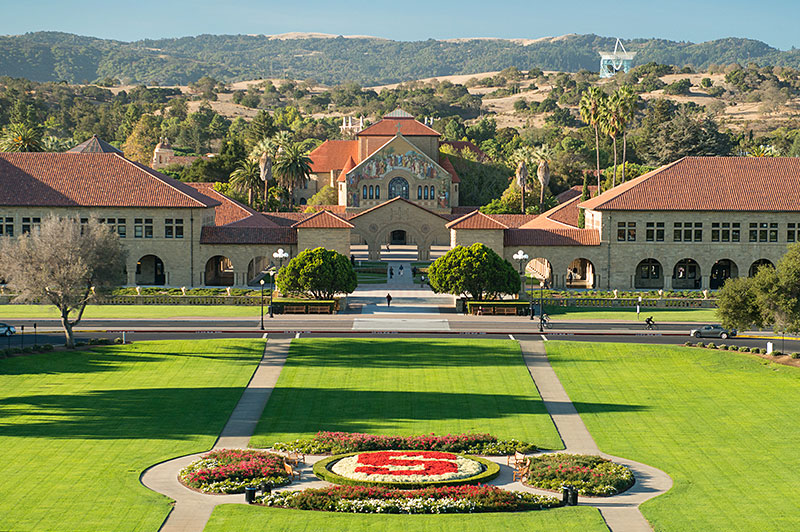
\includegraphics[width=0.9\textwidth]{fig/su}
  \label{fig:su}
\end{figure}

\begin{flushleft}
  The R Foundation Conference Committee\\
  The R Foundation for Statistical Computing\\
  c/o Institute for Statistics and Mathematics\\
  Wirtschaftsuniversit\"{a}t Wien\\
  Augasse 2-6\\
  1090 Wien, Austria\\
  Tel: (+43 1) 31336 4754\\
  Fax: (+43 1) 31336 774\\
  Email: \texttt{R-conferences@R-project.org}
\end{flushleft}


\date{\today}

\noindent To the R Foundation Conference Committee:

We are writing to propose that the campus of Stanford University,
Stanford California in the United States, be considered as a possible
venue for a future R User Conference (useR!). We would be especially
pleased to be considered as a possible host for the conference to be
held in the summer of 2016 as that would coincide with Dr.~John
Chambers 75th birthday and would mark a major milestone in the life
and contributions of an individual pivotal in the development of the R
language.


\section*{Location}

Stanford University is one of the world's leading research
universities. It is known for its entrepreneurial character, drawn
from the legacy of its founders, Jane and Leland Stanford, and its
relationship to Silicon Valley. Areas of excellence range from the
humanities to social sciences to engineering and the
sciences. Stanford is located in California's Bay Area, one of the
most intellectually dynamic and culturally diverse areas of the
nation. Established in 1885, the Stanford community includes 6,980
undergraduate students, 8,897 graduate students and 2,043 faculty
members which include 22 Nobel Laureates.

The Stanford campus is located on 8,180 contiguous acres is backed by
the Santa Cruz mountains to the West and the San Francisco Bay to the
East providing a host of scenic hiking, biking and other outdoor
activities. The majestic Pacific ocean is 24 miles to the West of the
the campus with opportunities to view birds, marine mammals and scenic
vistas. The Palo Alto downtown area is within walking distance of the
campus. A free shuttle bus service provides regular transportation to
downtown Palo Alto from multiple locations within the Stanford
Campus. Palo Alto provides a wide variety of restaurants including
Chinese, Indian, Central American, African, and Middle Eastern
cuisine.

Summer weather in Palo Alto is typically mild, sunny with a daily
average high of {26\celsius} and low of {14\celsius}, and average
humidity of 83\%.

\section*{Dates}

We propose to hold the conference over four days with tutorials
beginning on Monday, June 27, 2016.

\section*{Organization}

The following individuals comprise the conference organizational
committee:
\begin{itemize}
\item John M.~Chambers, \textsl{Stanford (Statistics)}
\item Sandrine~Dudoit, \textsl{Berkeley (Statistics)}
\item Trevor J.~Hastie, \textsl{Stanford (Statistics)}
\item Susan~Holmes, \textsl{Stanford (Statistics)}
\item Simon~D.~Jackman, \textsl{Stanford (Political Science)}
\item Olivia~Lau, \textsl{Google}
\item Nicholas~Lewin-Koh, \textsl{Genentech}
\item Norman~S.~Matloff, \textsl{UC Davis (Computer Science)}
\item Jacqueline~Meulman, \textsl{Stanford (Statistics)}
\item Balasubramanian~Narasimhan, \textsl{Stanford (Statistics)}
\item Karthik~Ram, \textsl{Berkeley (Institute for Data Science)}
\item Joseph~Rickert, \textsl{Revolution Analytics}
\item Duncan~Temple~Lang, \textsl{UC Davis (Statistics)}
\end{itemize}

Further members will be added as needed. We will enlist the support
of individuals through the Bay Area R Users Group (BARUG), local
industries, as well as Stanford and neighboring universities
(Berkeley, East Bay State, San Jose State, SF State, UCSF, and Davis).
Stanford has staff that can assist with meeting planning and
logistics, and the organizing team has already contacted them for
initial estimates and services.

BARUG is one of the most active R users associations in the world,
with a mailing list of over 3,400 Bay Area R users. It meets monthly,
typically at tech firms such as Google, Facebook, Dropbox and so on,
typically with two or three speakers at each meeting.  The presence of
BARUG adds further to the list of myriad reasons why the proposed
venue is perfect for UseR!.

\section*{Venue and Facilities}

The location of the conference will center on the Frances C. Arrillaga
Alumni Center which is located on the corner of Galvez and Campus
Drive. It is a comprehensive conference and event facility available
for events directly organized and conducted by a Stanford school or
department. With unique meeting rooms equipped with sound systems, an
elegant reception hall and beautiful outdoor gardens, the Alumni
Center has an auditorium that can seat a maximum of 600 people (McCaw
Hall) with adjacent breakout rooms in the Fisher Conference Center
that can be configured to provide, 6 rooms for 40 people each each or
4 rooms seating 80-100 people etc. In addition, the Koret-Taube
conference room in the adjacent
Gunn-SIEPR Building Center which can seat 120 people will be used for
focus sessions.

Facilities at the Alumni Center include
\begin{itemize}
\item Free Wi-Fi
\item Use of the Munzer Business Center with PCs, fax, copier, and printer
\item Access to The Alumni Caf\'e during normal business hours Monday
  through Friday
\item A dedicated event manager to help coordinate and oversee the
  conference
\item Front desk security for evening events
\item Up to two golf cart rentals, for a nominal fee
\item Convenient, nearby parking: the Track Lot or for large events,
  the rentable Galvez Lot.
\end{itemize}
The free Marguerite Shuttle conveniently stops in front of the Alumni
Center and can take conference attendees around campus or back to the
Palo Alto train station.

\subsection*{Capacities}
The floor plans and seating arrangements for McCaw Hall, Fisher
Conference Center and Koret-Taube Conference~Room 130 are shown in the
figures~\ref{fig:mccaw-fp}, \ref{fig:mccaw-seating},
\ref{fig:fisher-fp}, \ref{fig:koret-fp}. Table~\ref{tab:mc-capacity}
gives a comprehensive picture of the room capacities under varying
configurations.

\begin{figure}
  \centering
  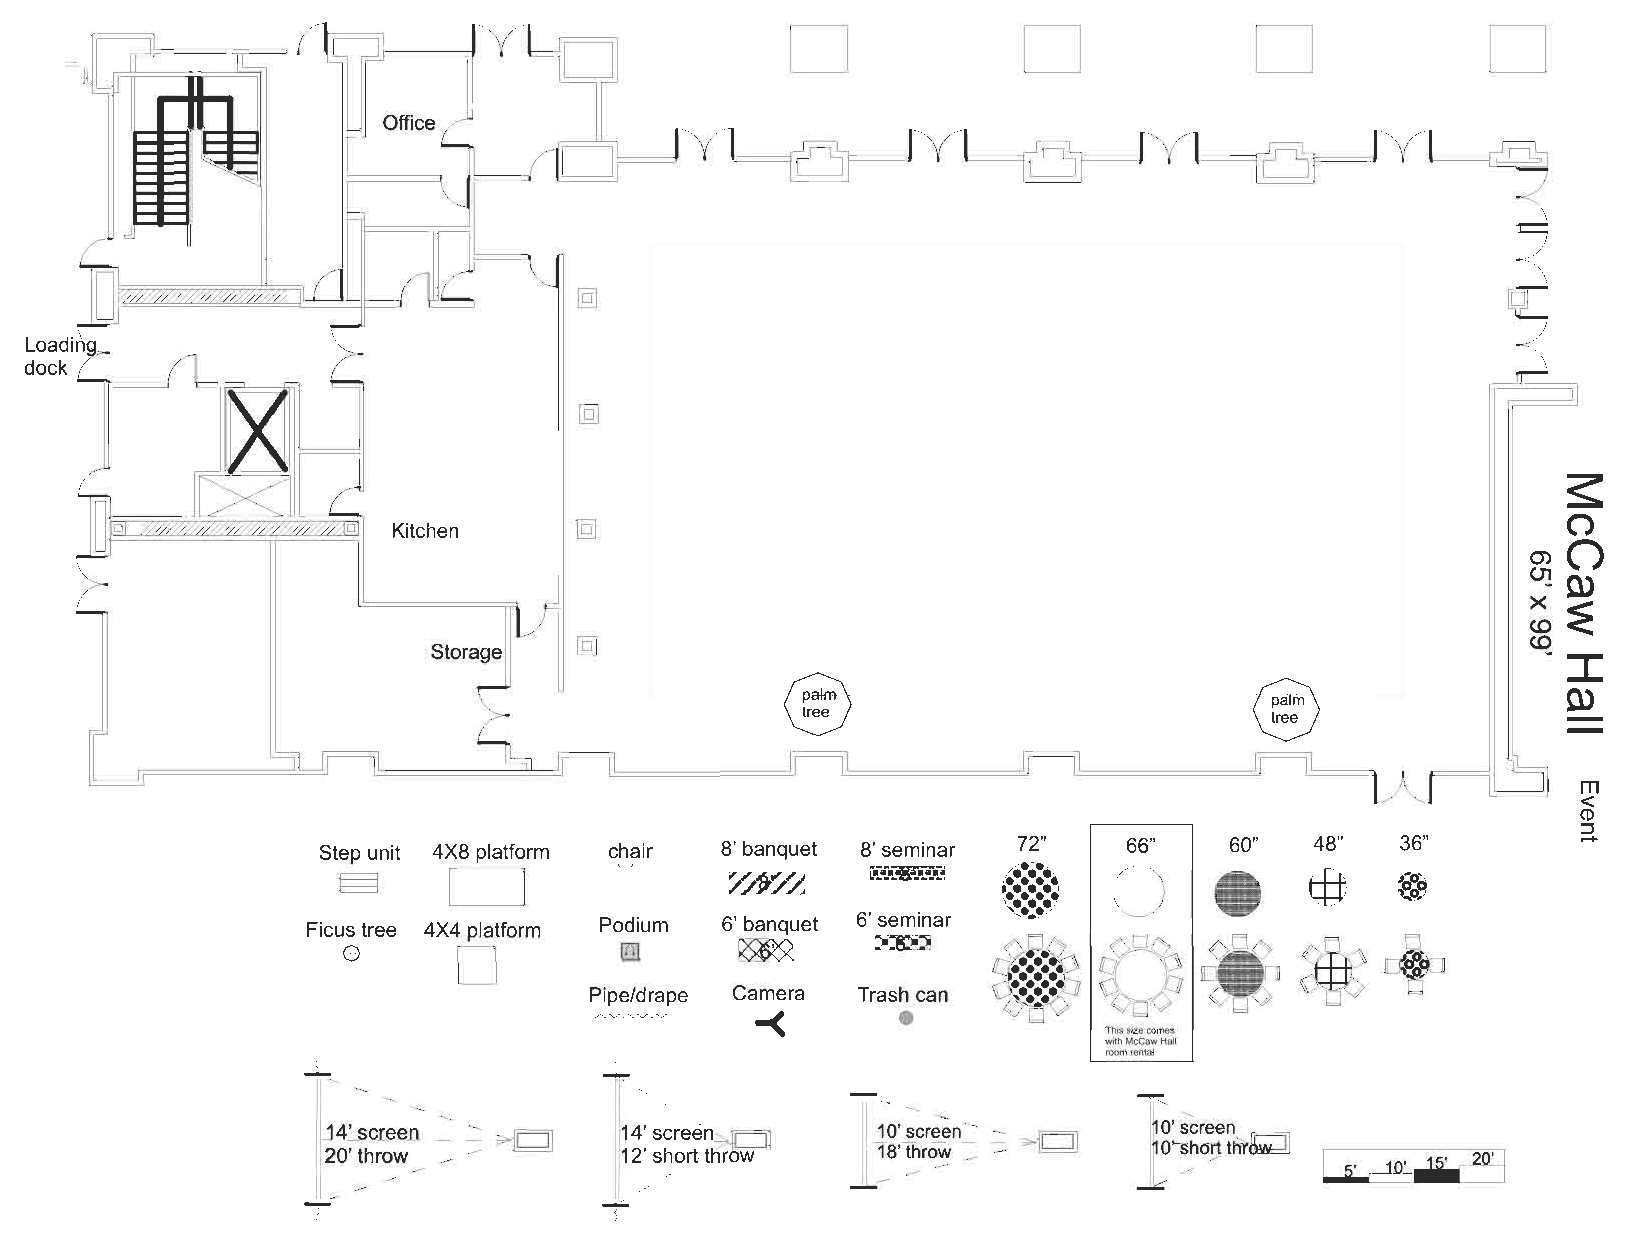
\includegraphics[width=0.98\textwidth]{fig/fpmccaw}
  \caption{McCaw Hall Floor Plan and Seating Styles}
  \label{fig:mccaw-fp}
\end{figure}

\begin{figure}
\centering
\begin{subfigure}{.5\textwidth}
  \centering
  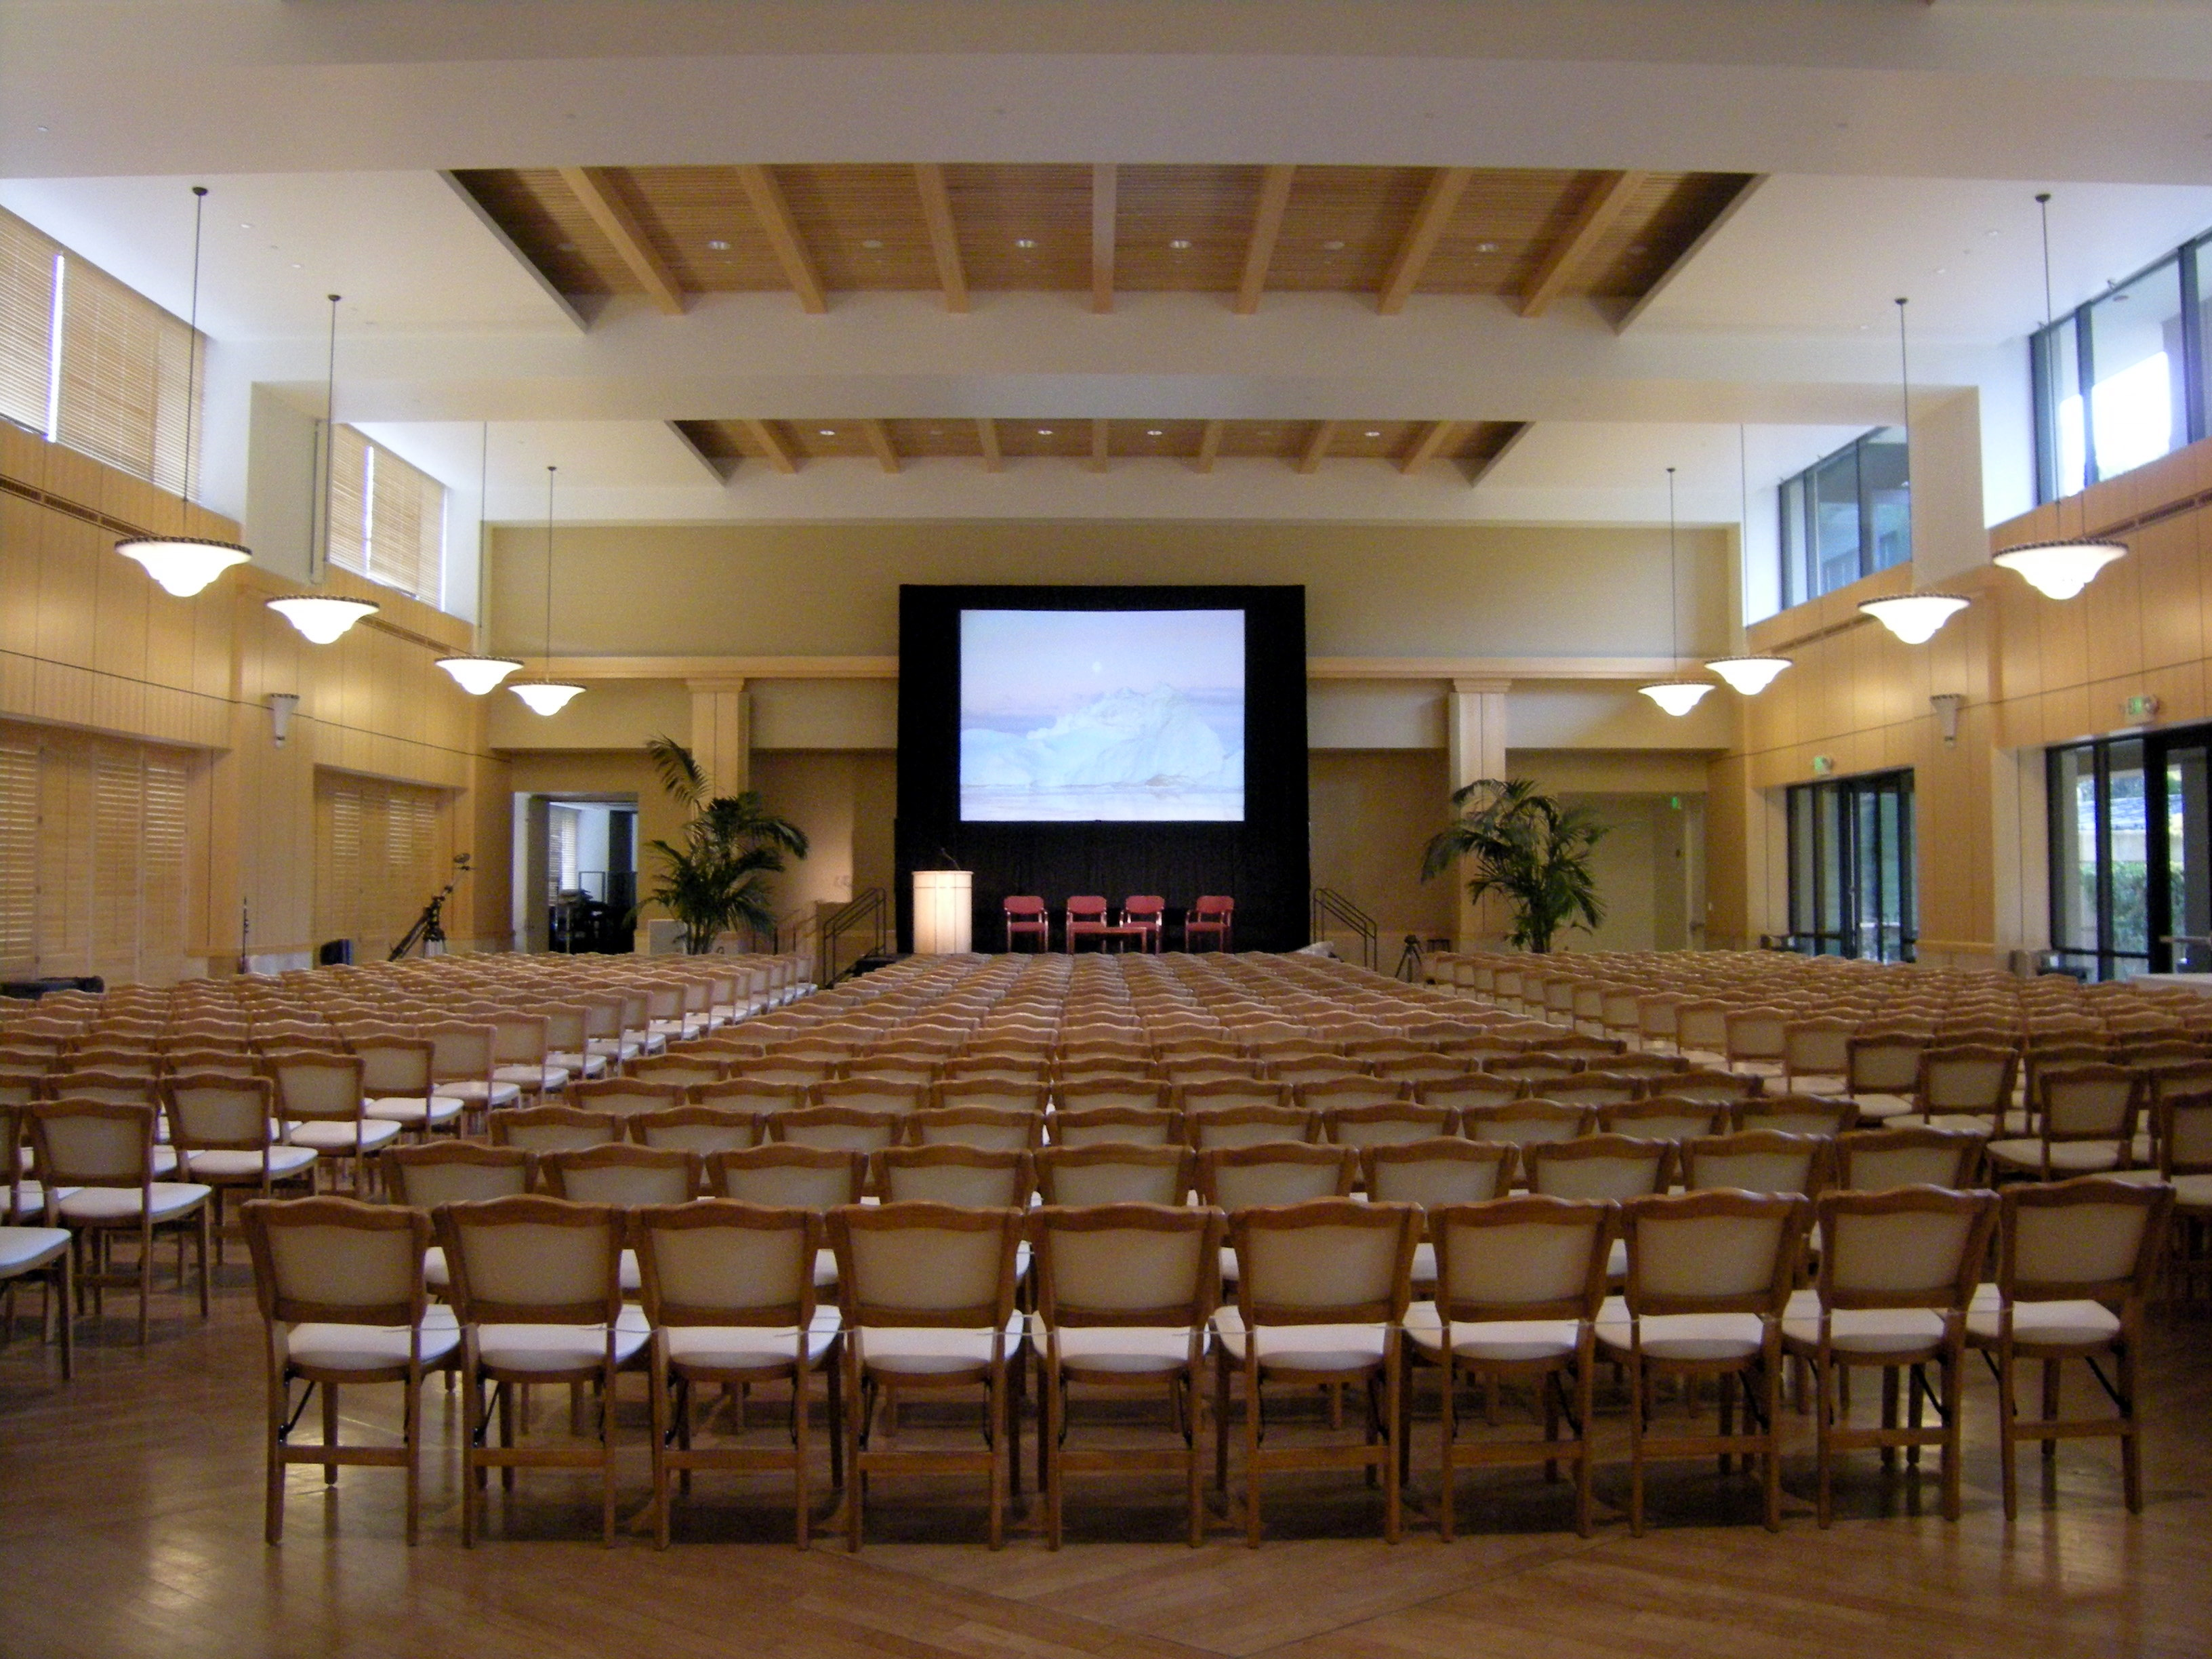
\includegraphics[width=.9\linewidth]{fig/mccawtheatre}
  \caption{McCaw Hall Arrangement 1}
  \label{fig:mccaw-theatre1}
\end{subfigure}%
\begin{subfigure}{.5\textwidth}
  \centering
  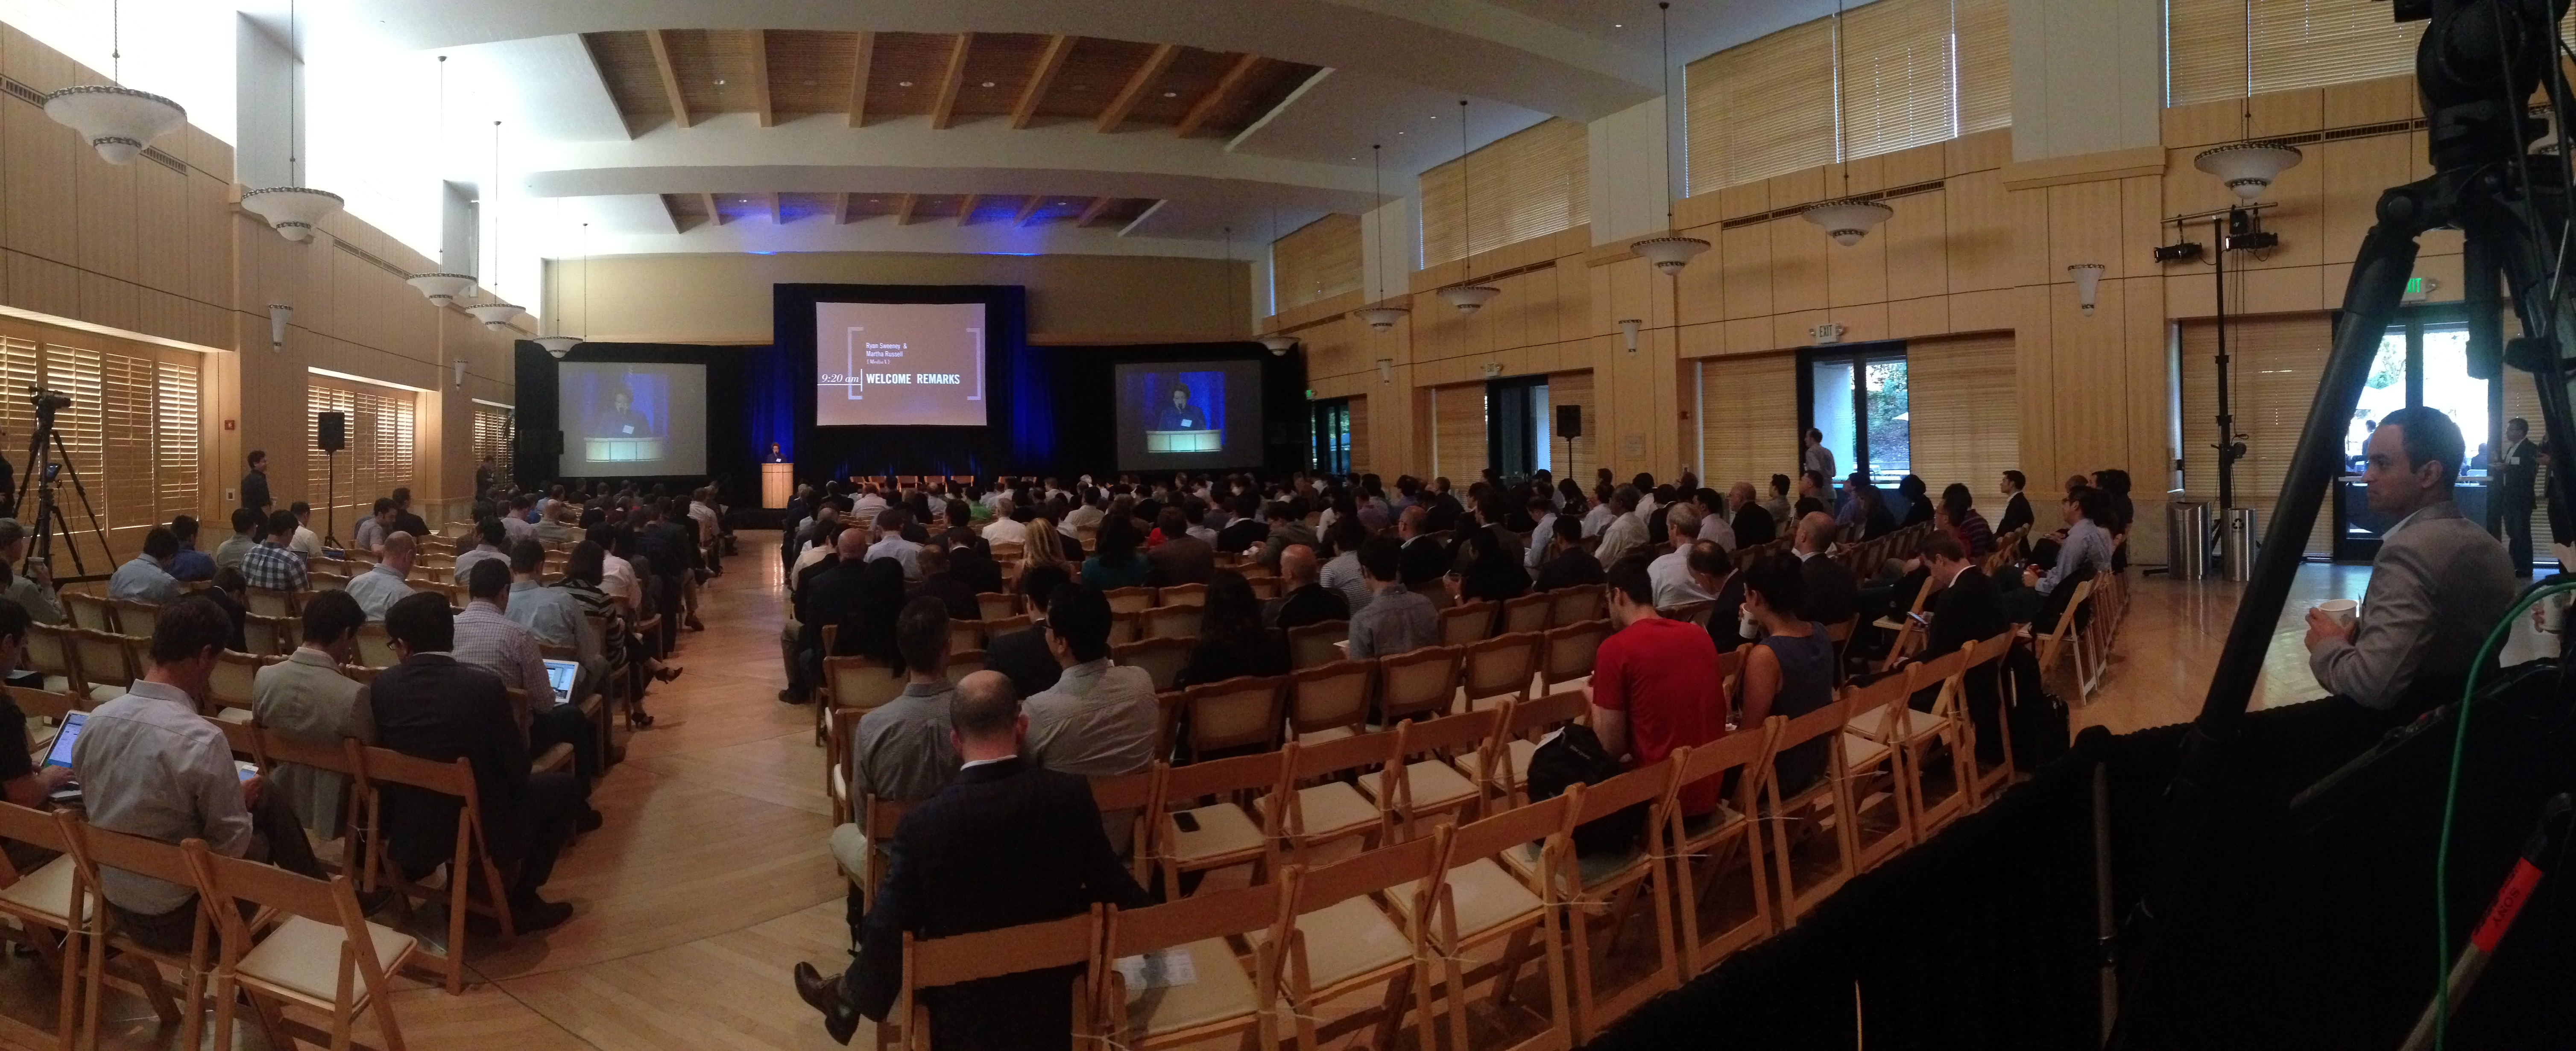
\includegraphics[width=.9\linewidth]{fig/mccawtheatre2}
  \caption{McCaw Hall Arrangement 2}
  \label{fig:mccaw-theatre2}
\end{subfigure}
\caption{McCaw Hall Seating Configurations}
\label{fig:mccaw-seating}
\end{figure}

\begin{figure}
\centering
\begin{subfigure}{.5\textwidth}
  \centering
  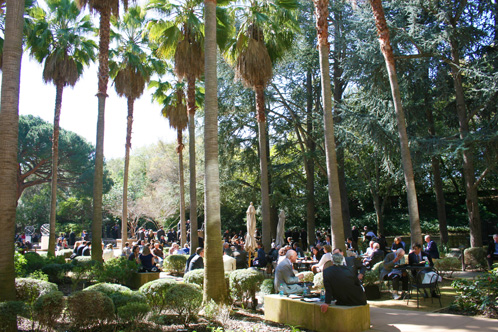
\includegraphics[width=.9\linewidth]{fig/palmct}
  \caption{Palm Court}
  \label{fig:palmct}
\end{subfigure}%
\begin{subfigure}{.5\textwidth}
  \centering
  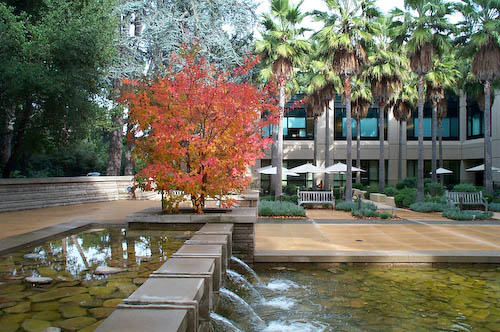
\includegraphics[width=.9\linewidth]{fig/palmfountain}
  \caption{Palm Court Fountain}
  \label{fig:palmfnt}
\end{subfigure}
\caption{Palm Court Area}
\label{fig:palm-court}
\end{figure}

\begin{figure}
\centering
\begin{subfigure}{.5\textwidth}
  \centering
  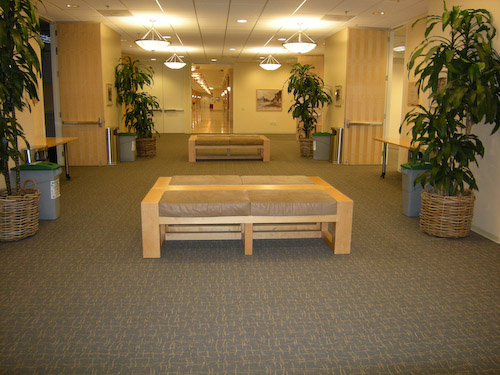
\includegraphics[width=.9\linewidth]{fig/fisher-foyer}
  \caption{Fisher Foyer}
  \label{fig:fisher-foyer}
\end{subfigure}%
\begin{subfigure}{.5\textwidth}
  \centering
  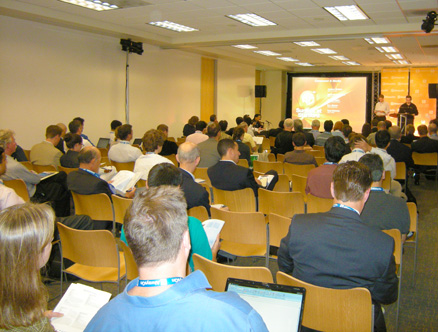
\includegraphics[width=.9\linewidth]{fig/fisher-class}
  \caption{Fisher Seating Arrangement}
  \label{fig:fisher-seat}
\end{subfigure}
\caption{Fisher Rooms and Foyer}
\label{fig:fisher-class}
\end{figure}


\begin{figure}
  \centering
  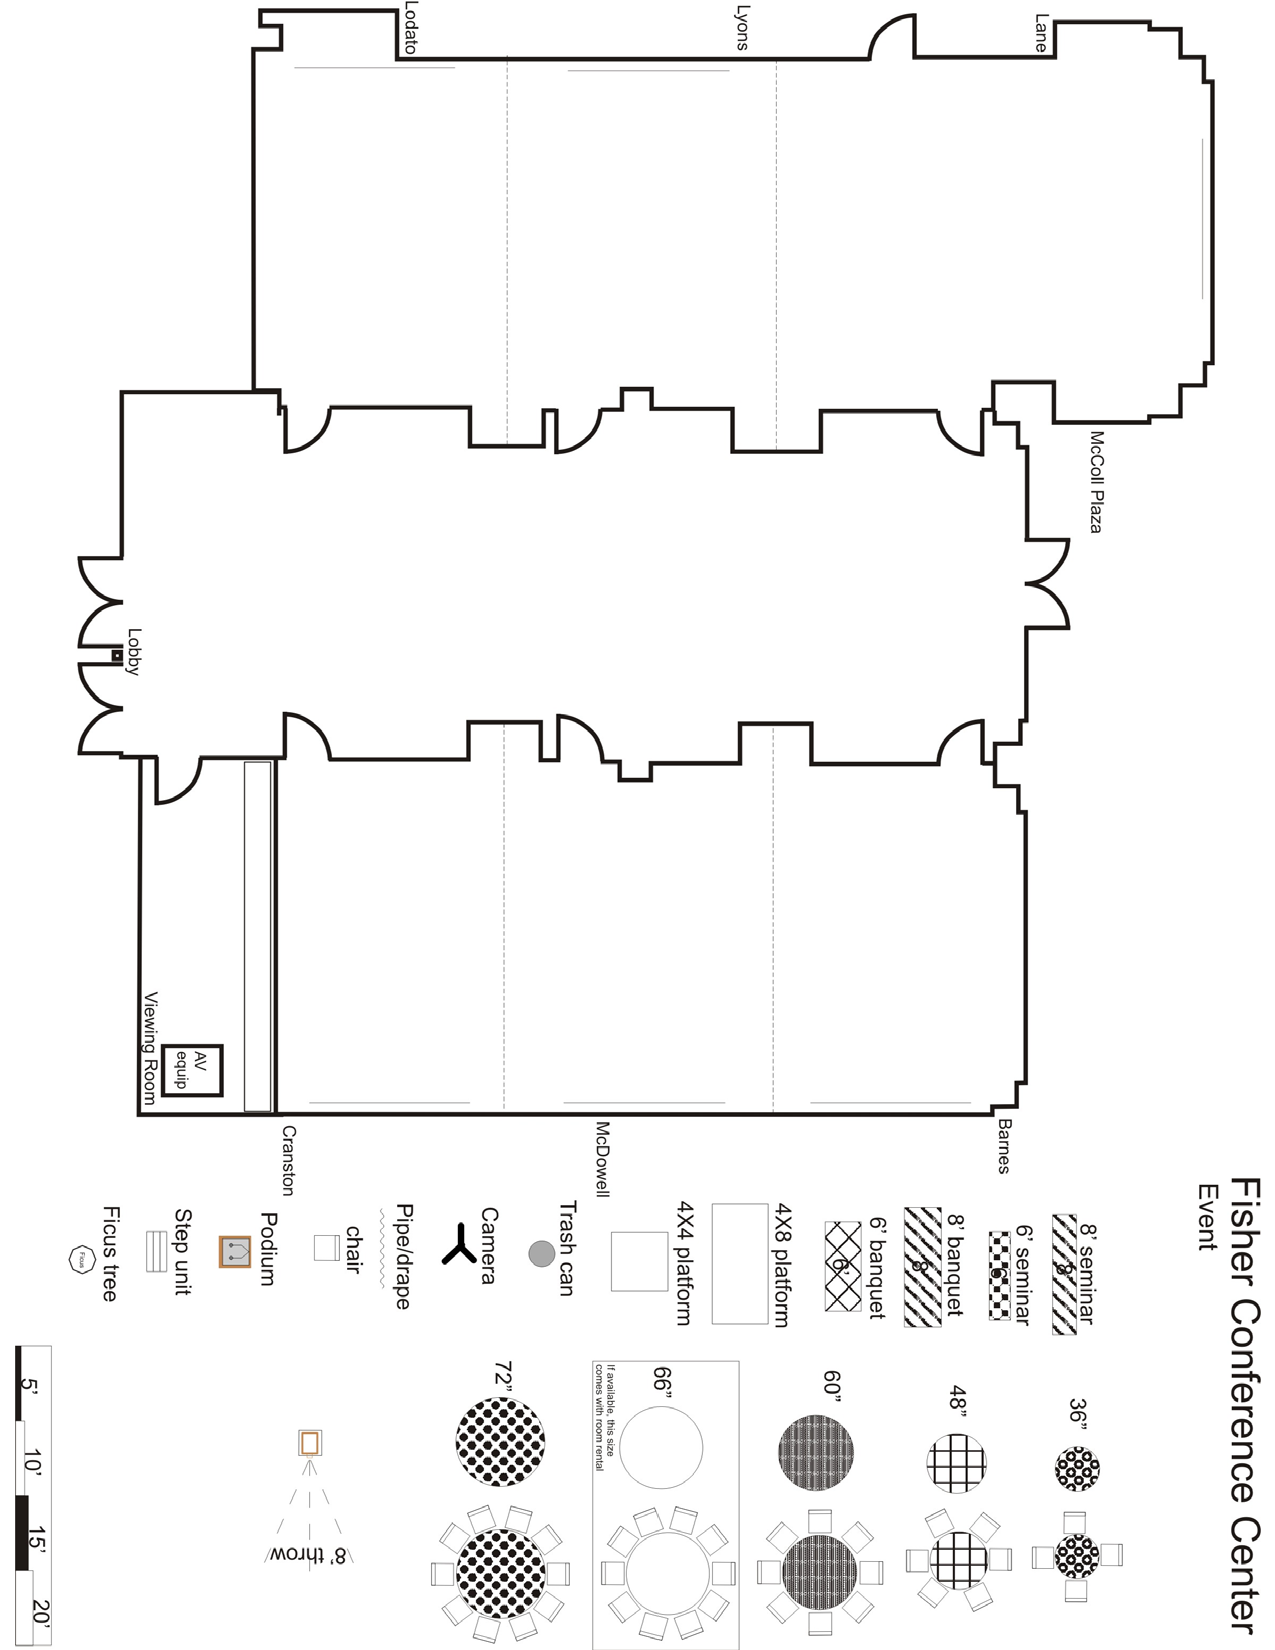
\includegraphics[width=0.98\textwidth]{fig/fpfisher}
  \caption{Fisher Rooms Floor Plan and Seating Styles}
  \label{fig:fisher-fp}
\end{figure}

\begin{figure}
  \centering
  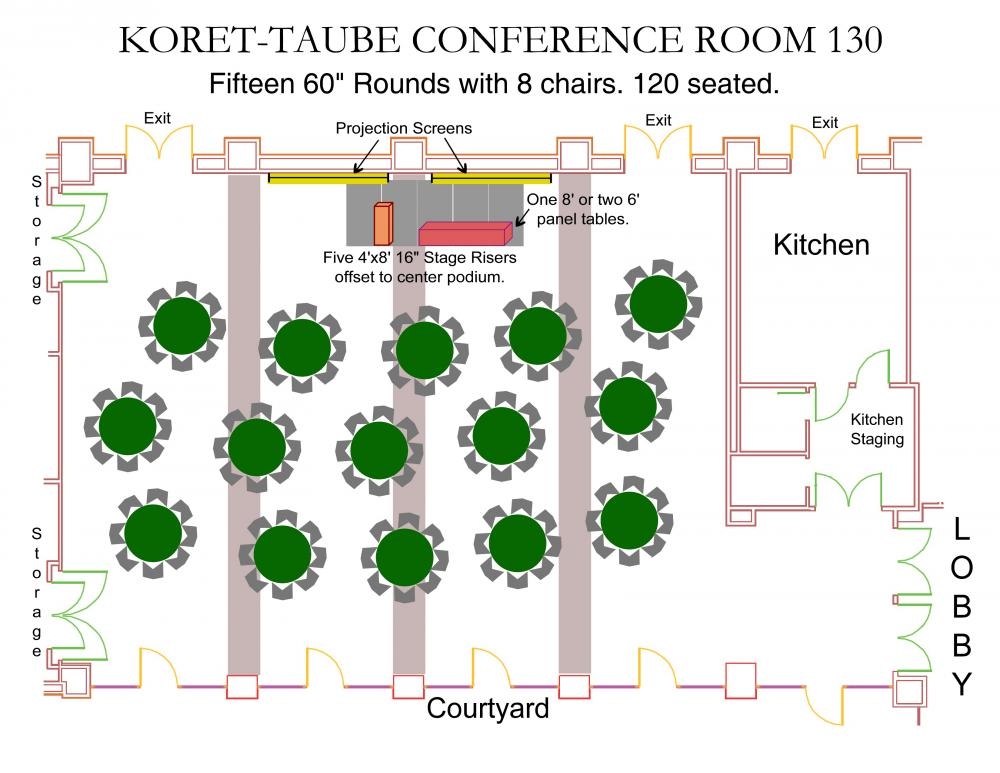
\includegraphics[width=0.98\textwidth]{fig/koret130}
  \caption{Koret Room 130 Floor Plan and Seating Styles}
  \label{fig:koret-fp}
\end{figure}

\begin{figure}
  \centering
  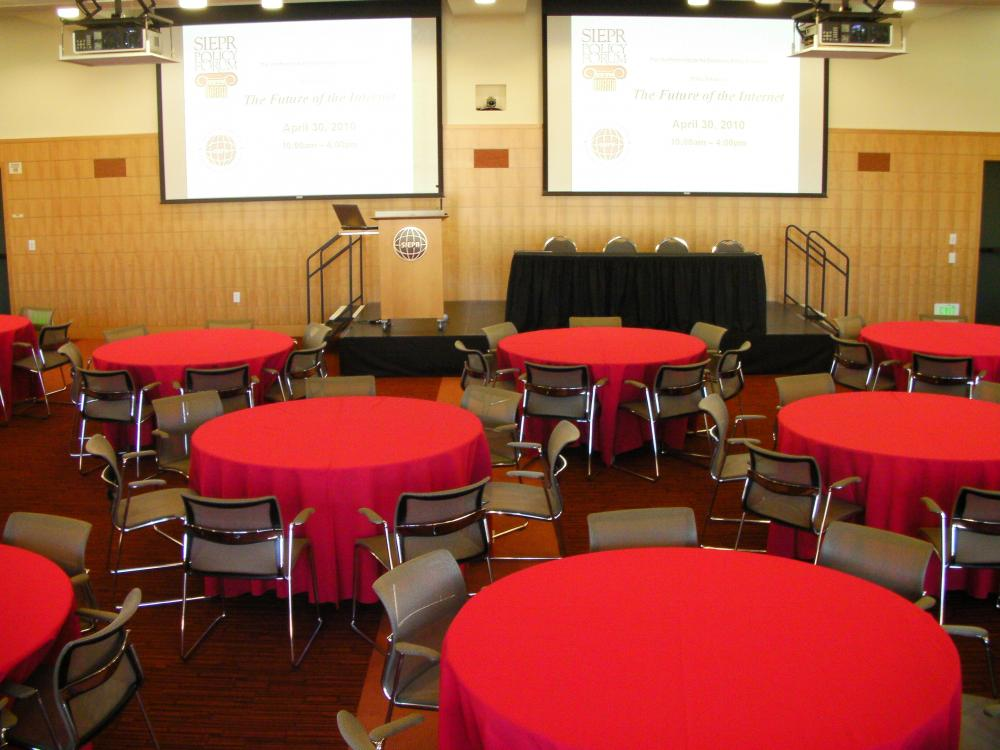
\includegraphics[width=0.5\textwidth]{fig/ktseat}
  \caption{Koret Room 130 Seating Arrangement}
  \label{fig:koret-seat}
\end{figure}

\begin{table}
  \centering
  \tiny
  %\begin{tabular}{lp{0.65in}p{0.3in}p{0.35in}p{0.65in}p{0.3in}p{0.3in}p{0.35in}l}
  \begin{tabular}{lcccccccc}
    \textbf{Venue}
    &\textbf{Dimensions (feet)}
    &\textbf{Area (sq.~ft.)}
    &\textbf{Theatre}
    &\textbf{Reception (standing)}
    &\textbf{U-Shape}
    &\textbf{Board Room}
    &\textbf{Dinner}
    &\textbf{Classroom}\\
    McCaw Hall & 99x65 &6435 &600 &942 &N/A &N/A &400 &250\\
    (Wooden Floor Area) &80x48 &3840 \\
    Lane &24x29 &696 &60 &60 &24 &26 &40 &36\\
    Lyons &24x18 &432 &40 &36 &15 &16 &20 &12\\
    Lodato &24x17 &408 &40 &36 &15 &16 &20 &12\\
    Lane \& Lyons &24x47 &1128 &100 &120 &39 &46 &40 &48\\
    Lyons \& Lodato &24x35 &840 &80 &100 &24 &36 &40 &24\\
    Lane \& Lyons \& Lodato &24x64 &1536 &150 &170 &63 &70 &100 &80\\
    Barnes &24x17 &408 &40 &36 &15 &16 &20 &18\\
    McDowell &24x18 &432 &40 &36 &15 &16 &20 &18\\
    Cranston &24x15 &375 &40 &36 &15 &16 &20 &9\\
    Barnes \& McDowell &24x35 &840 &80 &100 &24 &36 &40 &27\\
    McDowell \& Cranston &24x33 &792 &80 &100 &24 &36 &40 &27\\
    Barnes \& McDowell \& Cranston &24x50 &1200 &120 &140 &36 &50 &80
    &54\\
    Fisher Reception Area &50x17 &850 &N/A &100 &N/A &N/A &50 &N/A\\
    McColl &N/A &N/A &N/A &N/A &N/A &N/A &60-100 &N/A\\
  \end{tabular}
  \caption{McCaw Hall Capacities}
  \label{tab:mc-capacity}
\end{table}



\section*{Accommodation}
We are able to provide three levels of accommodation within close
proximity to the conference venue: business class hotels, budget
hotels and on-campus housing for students. Budget hotels run around
\$XXX/night and we hope to negotiate a group rate that will bring down
the cost for a four night stay to around \$XXX. On-campus housing is
cheaper although dependent on demand and length of stay. Current costs
for single dorm rooms run to about \$XX/night. Conference services at
Stanford with whom we have partnered will help us reserve a set of
on-campus dorm rooms.

\section*{Sponsorship and other financial support}
The Department of Statistics, Stanford University is sponsoring the
conference and is contributing funds towards the conference. In
addition, the Bay Area is home to companies known world-wide. Several
of them have already pledged verbal support and once our proposal is
approved formal arrangements will be set up. Income from corporate
sponsors and other sources is expected to be bounded below by \$XXK.

In addition, we expect to have stalls for companies to display/sell
books and related materials.

\section*{Budget}
The expected fixed costs are for the facility, conference room, IT
services, catering, security and administration. The catering includes
a welcome reception, coffee and lunch every day of the
conference. Table~\ref{table:regfees} shows the registration fees for
useR!~2012 (Vanderbilt University) and the useR!~2014 (UCLA) which are
at the two extremes. (There are some differences in what is included
in the registration fee, but that would be getting in the weeds.) We
expect our fees to be closer to the UCLA (more on that below).

\begin{table}[bhtp]
  \begin{tabular}{cccc}
    &\multicolumn{1}{c}{\textbf{Academic}}
    &\multicolumn{1}{c}{\textbf{Non-Academic}}
    &\multicolumn{1}{c}{\textbf{Student/Retiree}}\\
    Registration: Early & $(XXX, XXX)_{30\%}$ & $(XXX, XXX)_{15\%}$ & $(XXX, XXX)_{20\%}$\\
    Registration: Regular & $(XXX, XXX)_{15\%}$ & $(XXX, XXX)_{5\%}$ & $(XXX, XXX)_{5\%}$\\
    Registration: Late & $(XXX, XXX)_{5\%}$ & $(XXX, XXX)_{0\%}$ & $(XXX, XXX)_{5\%}$\\
    Registration: On-site & $(XXX, XXX)_{0\%}$ & $(XXX, XXX)_{0\%}$ & $(XXX, XXX)_{0\%}$\\
    Short Course & XXX & XXX & XXX\\
    Tutorial & XX & XXX & XX\\
  \end{tabular}
  \caption{Registration fees at recent useR!~conferences (2012,
    2014). Our assumed distributions are in subscripts.}
  \label{table:regfees}
\end{table}

The conference dinner costs an additional \$XXX/person.

\subsection*{Detailed Budget}

\paragraph{Tutorials}
\begin{center}
\begin{tabular}{lrr}
  \multicolumn{3}{c}{\textbf{Variable Budget (per person)}}\\
  \hline
  \multicolumn{1}{c}{Description}
  &\multicolumn{1}{c}{Income}
  &\multicolumn{1}{c}{Expense}\\
  \hline
  Tutorial fee (average fee) &XXX\\
  Meals, Lunch, coffee, tea:        & &XX\\
  Tutor fee (50\% of tutorial fee):             & &XX\\
  \hline
  \textbf{Total}             &XXX &XXX\\
  \hline
\end{tabular}
\end{center}

We expect a small surplus from the tutorials that will no doubt be
swallowed up by other expenses.


\paragraph{Conference}

\begin{center}
\begin{tabular}{lrr}
  \multicolumn{3}{c}{\textbf{Fixed Budget}}\\
  \hline
  \multicolumn{1}{c}{Description}
  &\multicolumn{1}{c}{Income}
  &\multicolumn{1}{c}{Expense}\\
  \hline
  Sponsorship &50,000\\
  Conference Hall (McCaw, 3 days) & &X,XXX\\
  Parallel Session Rooms (Fisher, 4 days) & &X,XXX\\
  Focus Session Room (Koret-Taub Room 130, 3 days) & &X,XXX\\
  Furniture/Audio Visual/Staff & &XX,XXX\\
  Ford Gardens (3 days, Outdoor Lunch/breaks) & &XXX\\
  Poster Session (Lawn, Umbrellas) & &X,XXX\\
  Mixer (Palm Court) & &XXX\\
  Invited speaker travel & &XX,XXX\\
  Gratis participants (sponsors, organizers) & &X,XXX\\
  \hline
  Total             &XX,XXX &XX,XXX\\
  \hline
  \textbf{Balance}             & &-XX,XXX\\
  \hline
\end{tabular}
\end{center}

The fixed costs are substantial and is expected to run us in the red
to the estimated amount of \$XX,XXX. However, we might have been
conservative in our estimate of corporate sponsorship.

\begin{center}
\begin{tabular}{lrr}
  \multicolumn{3}{c}{\textbf{Variable Budget (per person)}}\\
  \hline
  \multicolumn{1}{c}{Description}
  &\multicolumn{1}{c}{Income}
  &\multicolumn{1}{c}{Expense}\\
  \hline
  Avg.~Registration fee\footnotemark(2012, 2014) &(XXX, XXX) &XX\\
  Breakfast, coffee, tea, lunch (Tues-Thurs) & &XX\\
  Poster BBQ \& Bar & &XX\\
  Miscellaneous Expenses & &X\\
  Buffer & &5\\
  \hline
  Total             &(XXX, XXX)  &XXX\\
  \hline
  \textbf{Balance}             & &(XXX, XX)\\
  \hline
\end{tabular}
\footnotetext{Averages are computed using the assumed distribution in
  table~\ref{table:regfees}; fees used were those for the 2012 and
  2014 conferences.}
\end{center}

The surplus from the varying cost is \$XXX per registrant using the
2012 registration fees. Therefore, the break even point for the
conference is $XX,XXX/XXX\approx XXX$ participants. With 300, 400, 500
and 600 participants, the balances amount to \$XX,XXX, \$XX,XXX,
\$XX,XXX and \$XX,XXX respectively.

Using the 2014 numbers, the expected income per registration then
drops to approximately \$XXX. This brings down the the varying cost
surplus per registrant from \$XXX to \$XX. The break-even point goes
up to 347 registrants from 223. The surplus with 400, 500 and 600
registrants are \$X,XXX, \$XX,XXX and \$XX,XXX respectively.

Considering the reported attendance numbers for useR!~2014 (over 500),
we have good reason to expect that our registration fee would be close
to that of 2014.

\paragraph{Conference Dinner}
\begin{center}
\begin{tabular}{lrr}
  \multicolumn{3}{c}{\textbf{Variable Budget (per person)}}\\
  \hline
  \multicolumn{1}{c}{Description}
  &\multicolumn{1}{c}{Income}
  &\multicolumn{1}{c}{Expense}\\
  \hline
  Conference Dinner fee &XXX &\\
  Bus fee & &XX\\
  Meal, drinks, venue & &XXX\\
  \hline
  Total             &XXX &XXX\\
  \hline
  \textbf{Balance}             & &0\\
  \hline
\end{tabular}
\end{center}

The budget for the conference dinner should mostly balance itself.

\paragraph{Note}
Our budget was based on a detailed three-page estimate prepared by
Conference Planning Services at Stanford. They are highly experienced
and we have no reason to suspect their numbers. They quoted \$XXX per
head (venue, meals, drinks) and \$XX for the transporatation for
2014. So if the costs don't move much, we can bring this down to
\$XXX.

Finally, as remarked earlier, our sponsorship income estimate is
conservative. Our goal is really to break even while attracting as
large an audience as we can. Therefore, as the conference approaches
we will make every effort to lower the per participant registration
and conference dinner costs.

\section*{Scientific Program}

There is now a more or less stable format for useR!~contributions,
namely kaleidoscope talks, focus talks and lightning
presentions. We see no reason to deviate from this.

Some concern has been expressed that we have industry participation on
the conference committee. We plan to provide some guidelines for
session organizers so as to reduce the chance of overly commercial
talks. We also realize that we have to be creative about giving the
sponsors visibility. Therefore, we've noted this as an item for
discussion with the larger organizing committee---mostly academicians
we hasten to add---as we move forward in the process.

\section*{Social Program}
We envision providing three social events during the conference: an
on-campus welcoming reception on Monday night, a dinner on Wednesday
evening in the Palo Alto/Mountain View area and an outing to San
Francisco on Friday morning. Among the possible venues are the
Computer History Museum and the Mountain Winery.

\section*{Transportation}

Stanford is situated in Santa Clara County approximately 35 miles from
San Francisco and 20 miles from San Jose. The campus is accessible
from 3 international airports, San Francisco, San Jose and Oakland as
well as from interstate rail. Via Caltrain, Amtrak rail travelers can
reach Palo Alto by transferring trains in San Jose. The campus is
accessible locally via train (Caltrain), or the local bus systems SAM
trans and Santa Clara VTA.

Caltrain, the local commuter train, has a station in downtown Palo
Alto, and connects to the Bay Area Rapid Transit system (BART,
subway/light rail).  The BART connection makes travel to and from the
San Francisco airport easy, and enables convenient side trips for
attendees to visit San Francisco and Berkeley.

\section*{Campus Map}
\label{sec:campus-map}

Attached is a campus map that shows the location of the
Frances~C. Arrillaga Alumni Center (near Montag Hall) where the
conference will be hosted.

\begin{figure}
  \centering
  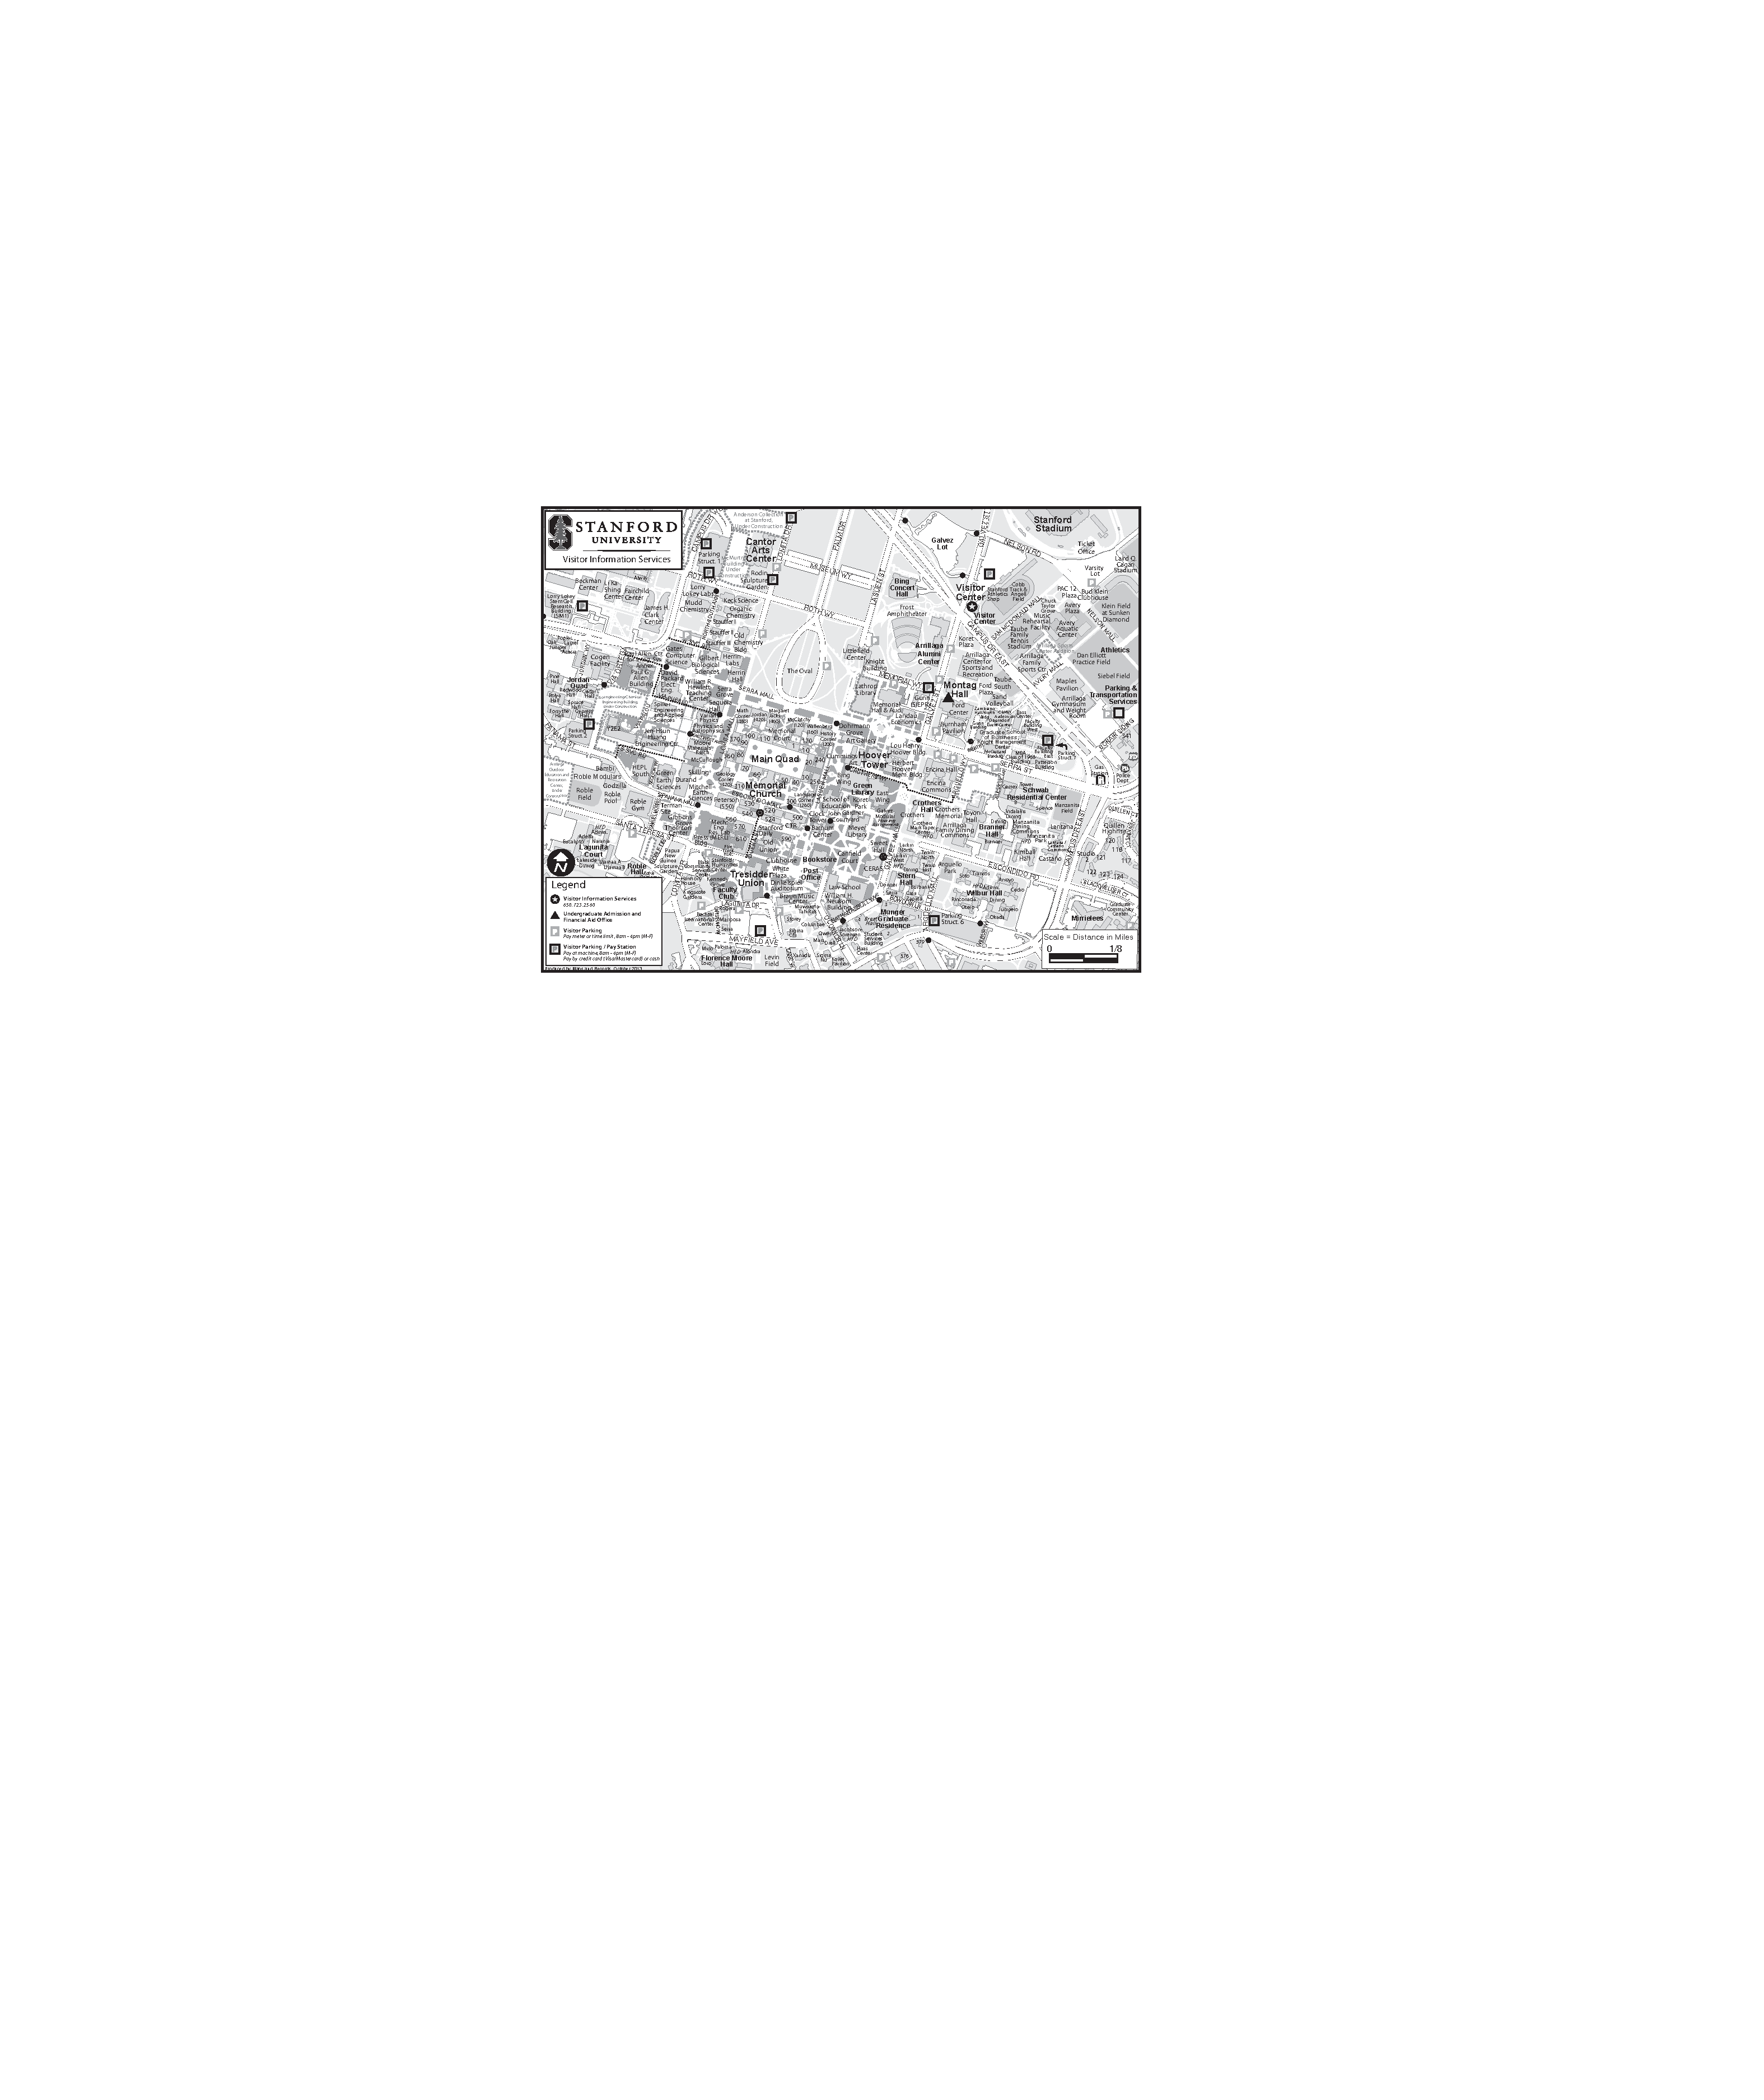
\includegraphics[width=0.98\textwidth]{fig/visitormap}
  \label{fig:campus-map}
\end{figure}

\end{document}